\chapter{C\# programming language}

Introduction \ref{sect01:imprv} presented the programming language C\# and its possible improvement of type inference. 
This chapter continues by describing relevant sections of the C\# language and its type inference algorithm to understand the possible barriers to implement improved type inference. 
Since type inference is a complicated process touching many areas of the C\# language, it firstly sorts these areas into separated groups described in necessary detail to understand all parts of the current type inference. 
These areas concern the C\# type system, including generics and language constructs where the type inference occurs or interacts with.

\section{Type system}

\begin{figure}[b]
\centering
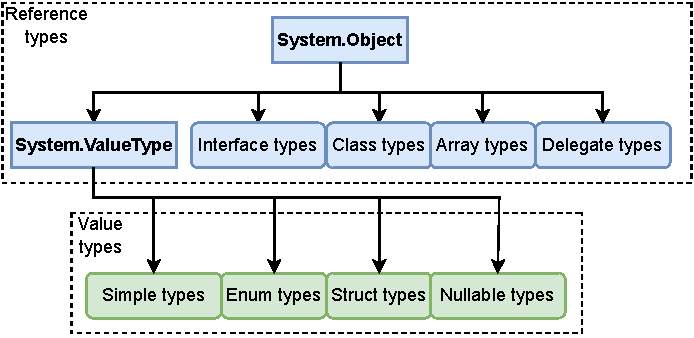
\includegraphics[width=140mm, height=65mm]{./img/CSTypeSystem.pdf}
\caption{The C\# data types schema adjusted from a C\# blog\cite{online:cSharpTypeSystem}.}
\label{img04:typeSys}
\end{figure}
C\# data types are defined in the C\# type system, which also defines relations between them. 
The most fundamental relation is type inheritance, where every type inherits another type, forming a tree with \texttt{System.Object} as a root node that doesn’t inherit any type.
Types are divided into value and reference types, shown in Figure 2.1, where an arrow means \textit{is inherited by} relation. 
Value types consist of built-in numeric types referred to as \textit{simple types}, and enumerations referred to as \textit{enum types}, structures referred to as \textit{struct types}, and nullable types. 
Compared to reference types, value types are implicitly sealed, meaning that they can’t be inherited by other types. 
Reference types consist of interfaces, classes, arrays, and delegates. 
An interface introduces a new relation to the type system by defining a list of methods, called a contract, which has to be implemented by a type that implements the interface.
The relation forms an acyclic graph, meaning a type can implement multiple interfaces, but the implementation relations can’t form a cycle. 
Delegates represent typed pointers to methods describing its signature, including generic parameters, parameters, and a return type.
\par
The type system implicitly allows to assign \texttt{null}, indicating an invalid value, to reference types. Since C\# 2.0 \cite{online:csHist}, it allows to assign \texttt{null} value to nullable types, which are equivalents of the rest of value types prohibiting it. Because assigning \texttt{null} value is referred to as a billion-dollar mistake, C\# 8.0 \cite{online:csHist}, introduced optional settings warning about assigning null values and created nullable reference types, which, together with nullable types, explicitly allows \texttt{null} assignment as a way of interaction with legacy code not using the feature.
\par
A big part of the type system is C\# \textit{generics}, allowing the parameterization of types and methods by arbitrary types. 
A specific generic method or type is \textit{constructed} by providing required type arguments, where \textit{construction} means replacing all occurrences of type parameters with the type arguments. 
Since type argument can be arbitrary type, the type parameter is considered to be the most general type in the type system, \texttt{System.Object}. 
Assuming additional API from the type parameter is achieved by restricting a set of types, which can replace the type parameter, enabling a specific interface of this set. 
The restriction is described by type constraints, which can be applied to type parameters. 
There are several kinds of constraints that can be combined together, forcing the type argument to fulfill all of them. 
Figure \ref{img05:typeConst} shows only two of them, and the rest can be found in the C\# documentation \cite{online:csharpTypeConst}. 
There is a definition of the \texttt{PrioritySorter} generic class with the \texttt{TItem} type parameter containing two constraints that the type argument has to hold. 
The \texttt{class} constraint allows only reference types. 
The \texttt{IPriorityGetter} constraint allows only types that implement the
interface.
\begin{figure}[h]
\begin{lstlisting}[style=csharp]
class PrioritySorter<TItem> where TItem : class, IPriorityGetter 
{ ... }
\end{lstlisting}
\caption{C\# type constraints.}
\label{img05:typeConst}
\end{figure}
\par
Constructed methods and types are new entities that don’t have any special relations between themselves implied from the construction. 
However, C\# generic interfaces can utilize a concept of type variance to introduce additional relations between constructed types. 
Initially, type parameters are \textit{invariant}, meaning an obligation to use the same type arguments as initially required. 
A type parameter can be specified to be \textit{covariant}, by prepending the type parameter declaration with the \texttt{in} keyword, allowing to use more derived type than initially required. 
0pposite \textit{contravariance} uses the \texttt{out} keyword, allowing to use
more general type than initially required.
\par
The last relevant feature of the type system is method overloading, which
allows definitions of multiple methods with the same name, return type, and count of type parameters having different types of parameters. 
Further chapters will mention the feature as an obstacle in designing efficient type inference.

\section{Relevant constructs}

Many unrelated C\# constructs can use type inference or can influence the type inference algorithm.
There are the most relevant whose internals are then considered in the following chapters regarding the design of the improvement.

\subsection*{Dynamic}

Introduction \ref{sect01:imprv} mentioned that strongly typed languages require knowing data types at compile time to prohibit incompatible operations on them. 
In the context of C\#, data means values of expressions that are transformed by operations defined on their types. 
It turned out that operations on expressions of unknown type at compile time became crucial for interoperability with other dynamic-typed languages whose types of expressions are known at runtime. 
To make the interoperability easier, C\# introduced the \texttt{dynamic} type that can be used as an ordinary type, which avoids the checks and causes \textit{dynamic binding}. 
\textit{Binding} is a process of resolving referenced operations based on the type and value of the expression. 
The majority of the C\# binding happens statically at compile time. Expressions containing a value of the \texttt{dynamic} type are dynamic bound at runtime, bypassing the static binding of the compiler. 
This behavior can lead to possible bugs regarding invalid operations on the dynamic data types, which will be reported during runtime. 
Figure \ref{img06:dynamic} shows a declaration of the \texttt{a} variable of the dynamic type.
Dynamic binding occurs in the \texttt{a.Foo()} expression, where the \texttt{Foo()} operation is not checked during compilation. 
An error is reported at runtime when the actual type of the \texttt{a} variable is determined to be \texttt{string}, which doesn’t define \texttt{Foo()} operation. Despite the dynamic binding, a compiler can still little check certain kinds of expressions containing values of dynamic types to reveal possible errors at compile time. 
An example of such checking is the \texttt{Bar()} method call, where the compiler can check the first argument, whose type is known at compile time as the type of the parameter. 
An appropriate error occurs during the compilation because string value has the \texttt{string} type, and it is passed as the \texttt{p1} parameter, which has the \texttt{int} type.
\begin{figure}[h]
\begin{lstlisting}[style=csharp]
dynamic a = "string";
a.Foo();
Bar("string", 1, a); \\ Compilation error reported

void Bar<T>(int p1, T p2, long p3) {...}
\end{lstlisting}
\caption{C\# dynamic type.}
\label{img06:dynamic}
\end{figure}

\subsection*{Anonymous function}

C\# allows to define a function without a name, called \textit{anonymous function}.
The function is represented as an expression that can be called or stored in a variable.
There are three types of anonymous function.
The first type is \textit{anonymous method} shown in Figure \ref{img06:anonymousF} where it is stored in the \texttt{a} variable.
The \texttt{b} variable contains the second type called \textit{explicit typed anonymous function}.
The third variable \texttt{c} contains the last type called \textit{implicit typed anonymous function}.
As can be seen, all of them have inferred return types based on return expression inside their bodies.
The most interesting type is the last one, where even parameter types are inferred based on a surrounding context and which is especially threatened by \textit{method type inference} algorithm mentioned in method type inference section \ref{sect02:MTIA}.
\begin{figure}[h]
\begin{lstlisting}[style=csharp]
Func<int, int> a = delegate(int p1) { return p1 + 1; };
Func<int, int> b = (int p1) => { return p1 + 1; };
Func<int, int> c = (p1) => { return p1 + 1; };
\end{lstlisting}
\caption{C\# anonymous functions.}
\label{img06:anonymousF}
\end{figure}

\subsection*{Object creation expression and initializer}

Initializers are used as a shortcut during an object instantiation.
The simplest one is \textit{object initializer} allowing to assign values to the object's fields pleasantly instead of assigning them separately after the initialization.
The second type of initializers regards arrays and collections.
\textit{Array initializers} are used to create fixed-size arrays with predefined content.
Figure \ref{img07:initializer} shows the \texttt{arrayInit} variable initialized by an array of \texttt{int} with two items using the initializer.
Under the hood, each item in the initializer is assigned to the corresponding index of the array after the array creation.
\textit{Collection initializers} are similar to array initializers defined on collections, which are created by implementing \texttt{ICollection<T>} interface.
One of the interface's declaring methods is \texttt{void Add<T>(T)} with adding semantics.
Each type implementing this interface is allowed to use an initializer list in the same manner as an array initializer.
It's just a sugar code hiding to call the \textit{Add} method for each item in the initializer list.
The last type of an initializer uses an indexer to store referred values on predefined positions, which is used in the second statement where the \texttt{indexerInit} variable is initialized by a dictionary object using indexers in its initializer list.
\begin{figure}[h]
\begin{lstlisting}[style=csharp]
var arrayInit = new int[] { 1, 2 };
var indexerInit = new Dictionary<string, int>() { 
    ["a"] = 1, ["b"] = 2 
};
\end{lstlisting}
\caption{C\# collection initializer.}
\label{img07:initializer}
\end{figure}

\section{Type inference} \label{sect02:typeInference}

C\# type inference occurs in many contexts. 
However, the proposed improvement will be inspired by and influence only a few of them.
These contexts are presented below.

\subsection{Keyword \texttt{var}}
One of the simplest type inference occurrences regards the \texttt{var} keyword used in a variable declaration.
It lets the compiler decide the type of variable based on the type of initializing value, which implies that it can’t use the keyword in declarations without initializing the value.
Figure \ref{img07:var} shows the usage, where the type of the \texttt{a} variable is determined to be \texttt{string} since it is initialized by a string value. 
\begin{figure}[h]
\begin{lstlisting}[style=csharp]
var a = "str";
\end{lstlisting}
\caption{Keyword \texttt{var}.}
\label{img07:var}
\end{figure}

\subsection{Operator \texttt{new()}}

There is also an opposite way of deducting types from a target to a source.
An example is the \texttt{new()} operator, which can be called with arbitrary arguments and represents object creation of a type that is determined by a type of the target. 
An example of these situations can be seen in Figure \ref{img08:new} where the target-typed \texttt{new(1)} operator allows to skip the specification of creating type in the object creation expression since the \texttt{myList} variable type gives it. After the type inference, the operator represents the new \texttt{new List<int>(1)} object creation expression.
\begin{figure}[h]
\begin{lstlisting}[style=csharp]
List<int> myList = new(1);
\end{lstlisting}
\caption{Operator \texttt{new()}.}
\label{img08:new}
\end{figure}

\subsection{Method type inference} \label{sect05:mti}

Method type inference is the most complex C\# type inference used during generic method call binding when type arguments are not given.
Figure \ref{img09:methodTypeInf} shows a situation when the method type inference deduces \texttt{System.String}, \texttt{System.Int32} and \texttt{System.Int32} as type arguments of the \texttt{Foo} method. 
There is a multi-step process that the type inference has to do to be able to infer it. 
Regarding the \texttt{T1} type parameter, the inference has to find a common type between the \texttt{(long)1} argument and the \texttt{(int)1} argument. 
Regarding the \texttt{T2} type parameter, the type inference has to go into type arguments of the generic type of the \texttt{p3} parameter and the \texttt{myList} argument, check if the types are compatible, and then match the \texttt{T2} type parameter against the \texttt{int} type argument of the \texttt{List<int>}. 
The \texttt{T3} type parameter is the most challenging since it occurs as a return type of the delegate. 
The type inference has first to infer types of input parameters of this delegate to be able to infer the implicit anonymous function’s return type. 
Then, it can match the inferred return type with the \texttt{T3} type parameter, resulting in the \texttt{System.Int32} type.
\begin{figure}[h]
\begin{lstlisting}[style=csharp]
List<int> myList = ...
Foo((long)1, (int)1, myList, (p1) => p1 + 1);

Foo<T1, T2, T3>(T1 p1, T1 p2, IList<T2> p3, Func<T2, T3> p4) {...}
\end{lstlisting}
\caption{Method type inference.}
\label{img09:methodTypeInf}
\end{figure}
\par
The method type inference algorithm is detailly described in separate section \ref{sect02:MTIA} since it is a complex algorithm, and the proposed improvement will be based on that.

\subsection{Array type inference}

The last mentioned type inference happens in array initializers when the array type should be deduced from the initializer list. 
Figure \ref{img14:arrayTypeInf} shows an example of a situation when the type inference is used for determining the \texttt{object[]} type of the \texttt{myArray} array. 
The C\# specification calls it \textit{common type inference}, which finds the most specialized common type between given types. 
From one point of view, it is just adjusted the method type inference algorithm where there is just one type variable, and all initializer items are lower bounds of that type variable.
\begin{figure}[h]
\begin{lstlisting}[style=csharp]
var myArray = new[] {new object(), "string"};
\end{lstlisting}
\caption{Array type inference.}
\label{img14:arrayTypeInf}
\end{figure}

\section{Method type inference algorithm} \label{sect02:MTIA}

Since one of the thesis's improvements is adjusting the algorithm, this section presents
its description. 
The thesis doesn’t show the complete algorithm described in the C\# specification \cite{online:csTypeInference} since it is complex, and some parts are unimportant for the following chapters. 
The simplified algorithm is divided into four subsections. 
The algorithm uses several definitions presented below.
\begin{defn}[Fixed type variables, bounds]
We call inferred type parameters \emph{type variables} which are at the beginning of the algorithm unknown, \emph{unfixed}. 
During the algorithm, they start to be restricted by sets of type \emph{bounds}.
The type variable becomes \emph{fixed} when the its actual type is determined using its \emph{bounds}.
\end{defn}
\begin{defn}[Method group]
A \emph{method group} is a set of overloaded methods resulting from a member lookup.
\end{defn}
\begin{defn}[Input/Output types]
If \texttt{E} is a method group or anonymous function and \texttt{T} is a delegate or expression tree type, then return type of \texttt{T} is an \emph{output type} of \texttt{E}.
If \texttt{E} is a method group or implicitly typed anonymous function, then all the parameter types of \texttt{T} are \emph{input types} of \texttt{E}. 
\end{defn}
\begin{defn}[Dependence]
An unfixed type variable \texttt{$X_i$} \emph{depends directly on} an unfixed type variable \texttt{$X_e$} if for some argument \texttt{E} \texttt{$X_e$} occurs in an input type of \texttt{E} and \texttt{$X_i$} occurs in an output type of \texttt{E}.
\texttt{$X_i$} \emph{depends on} \texttt{$X_e$} is the transitive but not reflexive closure of \emph{depends directly on}.
\end{defn}
\begin{table}[h]
\begin{center}
\begin{tabular}{ | l | l | } 
  \hline
  \texttt{\{Parameter\}.isValParam} & \makecell[lc]{Checks if the parameter is passed by\\ value.}\\ 
  \hline
  \texttt{\{Parameter\}.isRefParam} & \makecell[lc]{Checks if the parameter is passed by\\ reference.} \\ 
  \hline
  \texttt{\{Parameter\}.isOutParam} &\makecell[lc]{ Checks if the parameter has\\ \texttt{out} modifier.}\\ 
  \hline
  \texttt{\{Parameter\}.isInParam} & \makecell[lc]{Checks if the parameter has\\ \texttt{in} modifier.}\\ 
  \hline
  \texttt{\{Argument\}.isInArg} & \makecell[lc]{Checks if the argument has\\ \texttt{in} modifier.}\\ 
  \hline
  \texttt{\{Type\}.outTypes} & Returns \textit{Output} types of type.\\ 
  \hline
  \texttt{\{Type\}.inTypes} & Returns \textit{Input} types of type.\\ 
  \hline
  \texttt{\{Type\} isLike '\{Pattern\}'} & \makecell[lc]{Checks if the type matches\\ the pattern.}\\ 
  \hline
  \texttt{\{Type\}.isDelegateOrExprTreeType} & \makecell[lc]{Checks if the type is Delegate\\ or Expression Tree type.}\\ 
  \hline
\end{tabular}
\end{center}
\caption{Description of used properties.}
\label{table1:algorithmLegen}
\end{table}
\par
The pseudocode describing the algorithm uses custom helper functions explained in Table \ref{table1:algorithmLegen}.

\subsection{Algorithm phases}

Figure \ref{img10:methodTypeInference1} shows the initial phases of the algorithm. 
The method type inference process starts with receiving arguments of a method call and the method’s signature, which type parameters have to be deduced. 
The algorithm has two phases, where the first phase initializes initial bounds’ sets of type variables(inferred type arguments), and the second phase repeats until all type variables are fixed or fail if there is insufficient information to deduce them. 
Each type variable has three types of bounds. 
The exact bound consists of types, which have to be identical to the type variable, meaning that they can be converted to each other. 
The lower bound contains types that have to be convertible to the type variable, and the upper bound is opposite to it.
\begin{figure}[h!]
\begin{lstlisting}[style=myAlgo, mathescape=true]
Input: method call M($E_1$,...$E_x$) and 
       its signature $T_e$ M<$X_1$,...,$X_n$>($T_1$ $p_1$,...,$T_x$ $p_x$)
Output: inferred $X_1$,...$X_n$
  $B_{lower}$ = $B_{upper}$ = $B_{exact}$ = F = []
  FirstPhase()
  SecondPhase()

fn FirstPhase():
  E.foreach(e $\rightarrow$  
    if (e.isAnonymousFunc)
      InferExplicitParamterType(e, $T$[e.idx])
    elif (e.getType() is Type u)
      switch (u) {
        p[e.idx].isValParam $\rightarrow$ InferLowerBound(u, $T$[e.idx])
        p[e.idx].isRefParam || p[e.idx].isOutParam $\rightarrow$ 
          InferExact(u, $T$[e.idx])
        p[e.idx].isInParam && e.isInArg $\rightarrow$ 
          InferLowerBound(u, $T$[e.idx])
      }
  )
  
fn SecondPhase():
  while (true):
    $X_{indep}$ = $X$.filter(x $\rightarrow$ 
      F[x.idx] == null && $X$.any(x $\rightarrow$ dependsOn(x, y)))
    $X_{dep}$ = $X$.filter(x $\rightarrow$
      F[x.idx] == null && $X$.any(y $\rightarrow$ 
        dependsOn(y, x) && ($B_{lower}$+$B_{upper}$+$B_{exact}$).isNotEmpty))
    switch {
	  $X_{indep}$.isNotEmpty $\rightarrow$ $X_{indep}$.foreach(x $\rightarrow$ Fix(x))     
	  $X_{dep}$.isNotEmpty && $X_{indep}$.isEmpty $\rightarrow$ $X_{dep}$.foreach(x $\rightarrow$ Fix(x))
	  ($X_{indep}$+$X_{dep}$).isEmpty $\rightarrow$ 
	    return if (F.any(x $\rightarrow$ x == null)) Fail() else Success(F)
	  default $\rightarrow$ $E$.filter(e $\rightarrow$ 
	      $X$.any(x $\rightarrow$ 
	        F[x.idx] == null && $T$[e.idx].outTypes.contains(x)) 
	      && !X.any(x $\rightarrow$ 
	        F[x.idx] == null && $T$[e.idx].inTypes.contains(x))
	    ).foreach(e $\rightarrow$ InferOutputType(e, $T$[e.idx]))
    }
\end{lstlisting}
\caption{Phases of Method Type Inference}
\label{img10:methodTypeInference1}
\end{figure}
\par
\texttt{FirstPhase()} iterates over provided arguments and matches their types with types of corresponding parameters. 
This matching has two goals. 
The first is to check the compatibility of matched types, and the second is to collect the mentioned bounds associated with type variables contained in parameters’ types. 
This matching has many rules, followed by helping functions mentioned later in this section.
The matching represents dealing with the \texttt{T2} type parameter mentioned in Figure \ref{img09:methodTypeInf} where the compatibility between \texttt{List<int>} and \texttt{IList<T2>} is firstly checked, and then the \texttt{int} type is added as a lower bound of the \texttt{T2} type parameter. 
Type variables can have dependencies between themselves, so the first phase postpones matching output types of arguments’ types with corresponding parameters’ types because the output types can contain dependent type variables.
\par
\texttt{SecondPhase()} happens iteratively, respecting the \textit{depends on} relation.
Each iteration has two goals.
The first one is the fixation of at least one type variable.
If there is no type variable to fix because either all type variables are fixed or there are no other type bounds that could be used for type variable deduction, the algorithm ends.
The sets \texttt{$X_{indep}$} and \texttt{$X_{dep}$} refer to type variables, which can be fixed in the current iteration.
Line 31 contains the ending condition of the algorithm when all type variables are fixed, or there is no way to infer the next ones.
The second goal is to match postponed matching of output types of arguments' types with output types of corresponding parameters' types where all type variables in the output type of a parameter type don't depend on unfixed variable types contained in input types of the parameter type.
The second goal is to match postponed matching of output types of arguments' types with output types of corresponding parameters' types where all type variables in the output type of a parameter type don't depend on unfixed variable types contained in input types of the parameter type.
Line 32 describes this process using the pseudocode.
This goal represents dealing with implicit anonymous functions mentioned in Figure \ref{img09:methodTypeInf} where \texttt{T3} depends on \texttt{T2}.
The algorithm first infers the \texttt{T2} input type of the anonymous function, then infers the function's output type, which is then used to match the output type of \texttt{Func<T2, T3>} parameter type with the output type of the inferred anonymous function's type.
The match yields the \texttt{int} upper bound of the \texttt{T3} type parameter.

\subsection{Function type inference}

Figure \ref{img11:methodTypeInference2} contains definitions of two helper functions used in the first and second phases. 
The \texttt{ExplicitParameterType()} function is used to match an argument type, which is an explicit typed anonymous function. 
This function has typed parameters, so the algorithm matches them with input types of the corresponding parameter type.
\par
The \texttt{InferOutputType()} function is used in the second phase when postponed
matching of output types happens. 
Because potential type variables contained in the return types don’t depend on any unfixed type variables, the algorithm can match them. 
There are two situations where the output type is matched. 
The first situation regards anonymous functions, where the algorithm first infers the return type represented by the \texttt{InferReturnType()} function and then matches it with the output type of the corresponding parameter. 
The second situation regards method groups, which are firstly resolved by \texttt{OverloadResolution()}. 
The return type of the resolved method is matched with the output type of the corresponding parameter.
\begin{figure}[h!]
\begin{lstlisting}[style=myAlgo, mathescape=true]
fn InferExplicitParameterType(Argument E, Type T):
  if (E.isExplicitTypedAnonymousFunc && T.isDelegateOrExprTreeType
    && E.paramTypes.size == T.paramTypes.size)
      E.paramTypes.zip(T.paramTypes)
                  .foreach((e, t) $\rightarrow$ InferExact(e, t))
fn InferOutputType(Argument E, Type T):
  switch(E) {
	E.isAnonymousFunc && $T$.isDelegateOrExprTreeType $\rightarrow$
	  InferLower(InferReturnType(E), T.returnType) 
	E.isMethodGroup && T.isDelegateOrExprTreeType $\rightarrow$ {
	  	$E_{resolved}$= OverloadResolution(E, T.parameterTypes)
	  	if ($E_{resolved}$.size == 1) 
	  	  InferLower($E_{resolved}$[0].returnType, T.returnType) 
	  }
	E.isExpression && E.getType() is Type u $\rightarrow$ InferLower(u, T)
  }
\end{lstlisting}
\caption{\textit{Explicit parameter type inference}, \textit{Output type inference}}
\label{img11:methodTypeInference2}
\end{figure}
\newpage
\subsection{Collecting Type bounds}

\begin{figure}[h!]
\begin{lstlisting}[style=myAlgo, mathescape=true]
fn InferExact(Type U, Type V):
  if (Type t = X.find(x $\rightarrow$ V == x && F[x.idx] == null)) 
    $B_{exact}$[t.idx].add(U)
  switch(V) {
    V isLike '$V_1$[..]' && U isLike '$U_1$[..]' && V.rank == U.rank $\rightarrow$ 
      InferExact($U_1$, $V_1$)
    V isLike '$V_1$?' && U isLike '$U_1$' $\rightarrow$ InferExact($V_1$, $U_1$)
    V isLike 'C<$V_1,...,V_e$>' && U isLike 'C<$U_1,...,U_e$>' $\rightarrow$
      V.typeArgs.zip(U.typeArgs)
                .foreach((v, u) $\rightarrow$ InferExact(v, u)) 
  }
  
fn InferLower(Type U, Type V):
  if (Type t = X.find(x $\rightarrow$ V == x && F[x.idx] == null)) 
    $B_{lower}[t.idx]$.add(U)
  switch { .... }
  
fn InferUpper(Type U, Type V):
  if (Type t = X.find(x $\rightarrow$ V == x && F[x.idx] == null)) 
    $B_{upper}[t.idx]$.add(U)
  switch { ... }
\end{lstlisting}
\caption{\textit{Exact inference}, \textit{Upper-bound inference}, \textit{Lower-bound inference}}
\label{img12:methodTypeInference3}
\end{figure}
Figure \ref{img12:methodTypeInference3} shows three functions that add new bounds to type variables’
bound sets. 
Basically, all of them have similar behavior. 
It traverses the given \texttt{U} type contained in the argument type with the \texttt{V} type contained in the corresponding parameter type using the conditions contained in the \texttt{switch} statement and adds the \texttt{U} type to the type variable’s bound when the \texttt{V} type is a type variable. 
Since the branching conditions in \texttt{InferLower} and \texttt{InferUpper} are similar to those in \texttt{InferExact} and unimportant for the proposed improvement, the thesis omits it.
\par
\begin{obs}
There is no need to check possible contradictions because they are checked in the type variable fixation. 
\end{obs}
\begin{obs}
Bound sets don't contain unfixed type variables, which makes the algorithm simpler and which will be important for the following chapters.
The reason for that can be noticed in the design of functions API, where the left parameter always contains an expression or type from the argument, and the right parameter contains a type from the inferring method parameter. 
Since the three last-mentioned functions add only the type from the left parameter to bounds, there can’t be any type variables because argument types don’t contain type variables.
\end{obs}

\subsection{Fixation}

The last part of this algorithm is type variable fixation, shown in Figure \ref{img13:methodTypeInference4}. 
Initially, a set of candidates for the type variable is constructed by collecting all its bounds.
Then, it goes through each bound and removes the candidates who do not satisfy the bound’s restriction. 
If there is more than one candidate left, it tries to find a unique type that is identical to all left candidates. 
The fixation is successful if the candidate is found. 
The type variable is fixed to that type. 
This process can be seen in the initial example \ref{img09:methodTypeInf}, where the \texttt{T1} type variable contains \texttt{long} and \texttt{int} in its lower bound set. 
At the start of this process, both types are candidates. 
However, \texttt{int} is removed because it doesn’t have an implicit conversion to \texttt{long}.
\par
\begin{figure}[h!]
\begin{lstlisting}[style=myAlgo, mathescape=true]
fn Fix(TypeParameter x):
  $U_{candidates}$ = $B_{lower}$[x.idx] + $B_{upper}$[x.idx] + $B_{exact}$[x.idx]
  $B_{exact}$[x.idx].foreach{b $\rightarrow$ 
    $U_{candidates}$.removeAll(u -> !b.isIdenticalTo(u))}
  $B_{lower}$[x.idx].foreach{b $\rightarrow$ 
    $U_{candidates}$.removeAll(u -> !hasImplicitConversion(b, u))}
  $B_{upper}$[x.idx].foreach{b $\rightarrow$ 
    $U_{candidates}$.removeAll(u -> !hasImplicitConversion(u, b))}
  temp = $U_{candidates}$.filter(x $\rightarrow$ $U_{candidates}$.all(y $\rightarrow$ 
    hasImplicitConversion(y, x)))
  if (temp.size == 1) F[i] = temp[0] else Fail()
\end{lstlisting}
\caption{Fixing of type variables}
\label{img13:methodTypeInference4}
\end{figure}
\par
An important observation of the method type inference is an obligation of infering all type arguments of the method.
If the compiler is not able to infer all type arguments, an user has to specify all type arguments.
C\# currently doesn't offer a way how to hint just ambigious type arguments.